\subsection{Etude du lien entre le temps d'études et le sommeil}

\subsubsection{Tableau de contingence et test chi-deux pour l'ensemble des individus}

Nous avons aussi voulu étudier le lien entre le temps que consacre les étudiants pour leurs études par jour et leurs temps de sommeil.
Pour commencer nous pouvons voir avec le tableaux de contingence en figure \ref{tab:contTableStudySleepAll} que si on prends l'ensemble des individus alors la répartition dans chaque catégorie est suffisante pour avoir une analyse cohérente. 

\begin{figure}[!h]
    \begin{center}
      \begin{tabular}{|c|c|c|c|c|}
        \hline 
        & \multicolumn{4}{|c|}{sleep duration}\\ 
        \hline
        study hours & 5-6 hours & 7-8 hours & Less than 5 hours & More than 8 hours\\ 
        \hline 
        3- & 20 & 28 & 25 & 27\\ 
        \hline 
        3-6 & 22 & 24 & 31 & 29\\ 
        \hline 
        6-9 & 24 & 31 & 26 & 42\\ 
        \hline 
        9+ & 57 & 45 & 41 & 30 \\ 
        \hline
      \end{tabular}
    \end{center}
    \caption{Table de contingence entre le temps consacré par jour aux études et le temps de sommeil}
    \label{tab:contTableStudySleepAll}
\end{figure}

Nous avons ensuite réalisé un test Chi-deux pour être sûre que l'AFC est du sens. La p-valeur obtenue est de $\approx3,2\%$ ce qui est suffisant pour montré une corrélation entre les deux valeurs.

\subsubsection{Tableau de contingence et test chi-deux pour les individus dépressifs et non dépressifs}

Si on limite l'analyse seulement aux individus non dépressifs on obtient la table de contingence en figure \ref{tab:contTableStudySleepNonDepressive}.
Cette limitation fait disparaitre la corrélation entre les deux variables. 
En effet, la p-valeurs est de $\approx13,6\%$ ce qui est bien supérieur aux valeurs nécessaires pour qu'une corrélation soit observé.
   
\begin{figure}[!h]
    \begin{center}
        \begin{tabular}{|c|c|c|c|c|}
        \hline 
        & \multicolumn{4}{|c|}{sleep duration}\\ 
        \hline
        study hours & 5-6 hours & 7-8 hours & Less than 5 hours & More than 8 hours\\ 
        \hline 
        3- & 12 & 18 & 19 & 18\\ 
        \hline 
        3-6 & 16 & 10 & 16 & 16\\ 
        \hline 
        6-9 & 7 & 14 & 13 & 20\\ 
        \hline 
        9+ & 24 & 19 & 11 & 17 \\ 
        \hline
        \end{tabular}
    \end{center}
    \caption{Table de contingence entre le temps consacré par jour aux études et le temps de sommeil par les individus non depressifs}
    \label{tab:contTableStudySleepNonDepressive}
\end{figure}

Ensuite, si on limite seulement aux individus dépressifs on obtient le tableau de contingence en figure \ref{tab:contTableStudySleepDepressive}.
On voit que de la même que pour les individus non dépressifs la corrélation disparait.
La p-valeurs est de $\approx5,8\%$ ce qui est assez proche des valeurs prisent pour indiquer une faible corrélation qui n'est pas aussi forte qu'avec tous les individus sans distinctions. 

\begin{figure}[!h]
    \begin{center}
    \begin{tabular}{|c|c|c|c|c|}
        \hline 
        & \multicolumn{4}{|c|}{sleep duration}\\ 
        \hline
        study hours & 5-6 hours & 7-8 hours & Less than 5 hours & More than 8 hours\\ 
        \hline 
        3- & 8 & 10 & 6 & 9\\ 
        \hline 
        3-6 & 6 & 14 & 15 & 13\\ 
        \hline 
        6-9 & 17 & 17 & 13 & 22\\ 
        \hline 
        9+ & 33 & 26 & 30 & 13 \\ 
        \hline
    \end{tabular}
    \end{center}
    \caption{Table de contingence entre le temps consacré par jour aux études et le temps de sommeil par les individus depressifs}
    \label{tab:contTableStudySleepDepressive}
\end{figure}

Pour résumer, il n'y pas de corrélation entre le temps consacré aux études et la durée du sommeil lorsque nous observons un groupe restreint d'individu (dépressifs et non dépressifs).
Nous observons donc un inversement de la tendance lorsque nous prennons les individus dans leur totalité.
Ce phénomène s'apparente encore une fois au paradoxe de Simpson \citep{simpson}. Il peut s'expliquer par une troisième variable affectée par ce choix de séparé les individus dépressifs et non dépressifs.

\subsubsection{Valeurs propres et cercle de corrélations}
 
Après avoir réalisé l'AFC, on obtient le cercle de corrélation en figure \ref{fig:corrStudySleep}. 
Nous trouvons que les deux composantes principales explique $\approx96,5\%$ de la variance avec en particulier la première qui en explique $\approx84,9\%$.
Il faut donc regardé en priorité l'axe des abscisses pour chercher des corrélations.


\begin{figure}[H]
    \begin{center}
      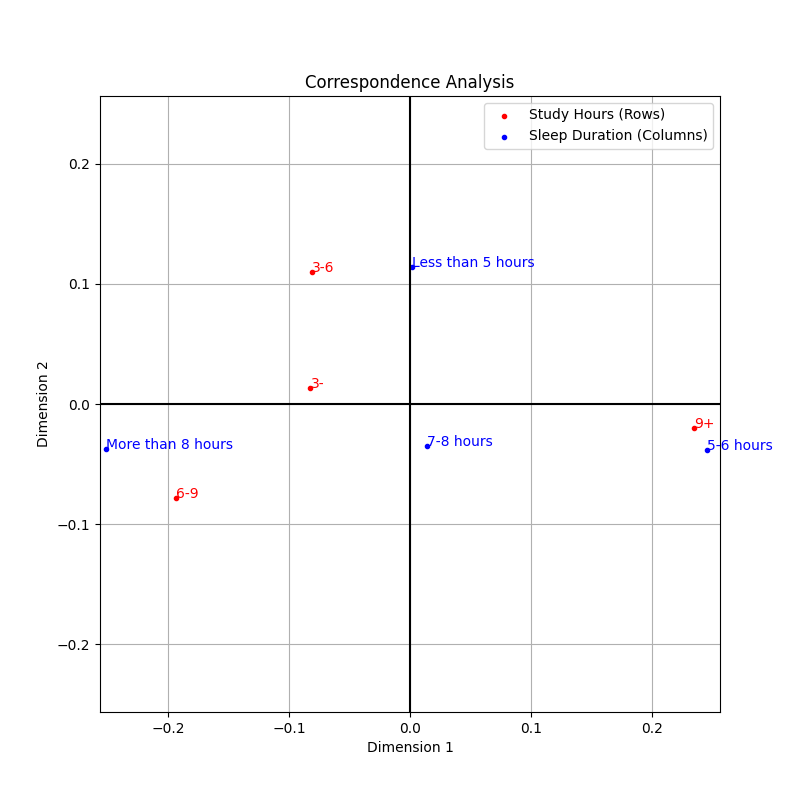
\includegraphics[width=0.55\textwidth,height=0.325\textheight,keepaspectratio]{Images/Study_Sleep_all/Corr_circle.png}
    \end{center}
    \caption{Cercle des corrélations de l'AFC sur le temps d'études et le temps de sommeil}
    \label{fig:corrStudySleep}
\end{figure}

C'est ainsi que nous remarquons deux tendances. 
En effet, nous remarquons que les étudiants travaillant le plus, c'est à dire 9 heures ou plus, ont tendance à dormir entre 5 et 6 heures. 
Cette tendance s'explique facilement, les étudiants travaillant beaucoup passe moins de temps à dormir car ils utilisent leurs temps pour travailler.
Ces étudiants n'ont pas les durées de sommeil les plus courtes non plus car ce comportement corresponds à des étudiants passant beaucoup de temps à travailler mais aussi à des étudiants ayant des comportement différentes ou étant dans des situations particulières comme par exemples des étudiants victime d'insomnie.

Le cercle de corrélation montre aussi une deuxième tendance, celle-ci un plus faible que la première.
En effet, on remarque que les étudiants dormant plus de 8h ont tendance à travailler entre 6 et 9 heures.
Ces étudiants travaille beaucoup, deuxième catégorie avec la plus grosse durée de travail, mais ont aussi le temps de sommeil le plus long.
Cela peut s'expliquer par des étudiants gérant mieux leurs temps en travaillant beaucoup sans avoir à perdre du temps de sommeil.


Cette tendance est confirmé par la figure \ref{fig:contribStudySleep}.
Nous remarquons qu'en accord avec la figure \ref{fig:corrStudySleep} les catégories contribuant le plus à la première composante sont 5-6 hours et More than 8 hours de manière approximativement égale pour le temps de sommeil.
Nous retrouvons pour le temps consacré aux études que les catégories contribuant le plus sont bien 9+ et 6-9, mais avec un écart bien plus important entre les contribution de ces catégories.
Ensuite, pour la deuxième composante nous remarquons la catégorie 6-9 qui a une contribution assez élévé et nous retrouvons aussi des catégories dont nous n'avons pas tiré de corrélation.
Ce qui s'explique par le fait que la seconde composante n'explique que $\approx11,6\%$ de la variance.

\begin{figure}[H]
    \begin{center}
      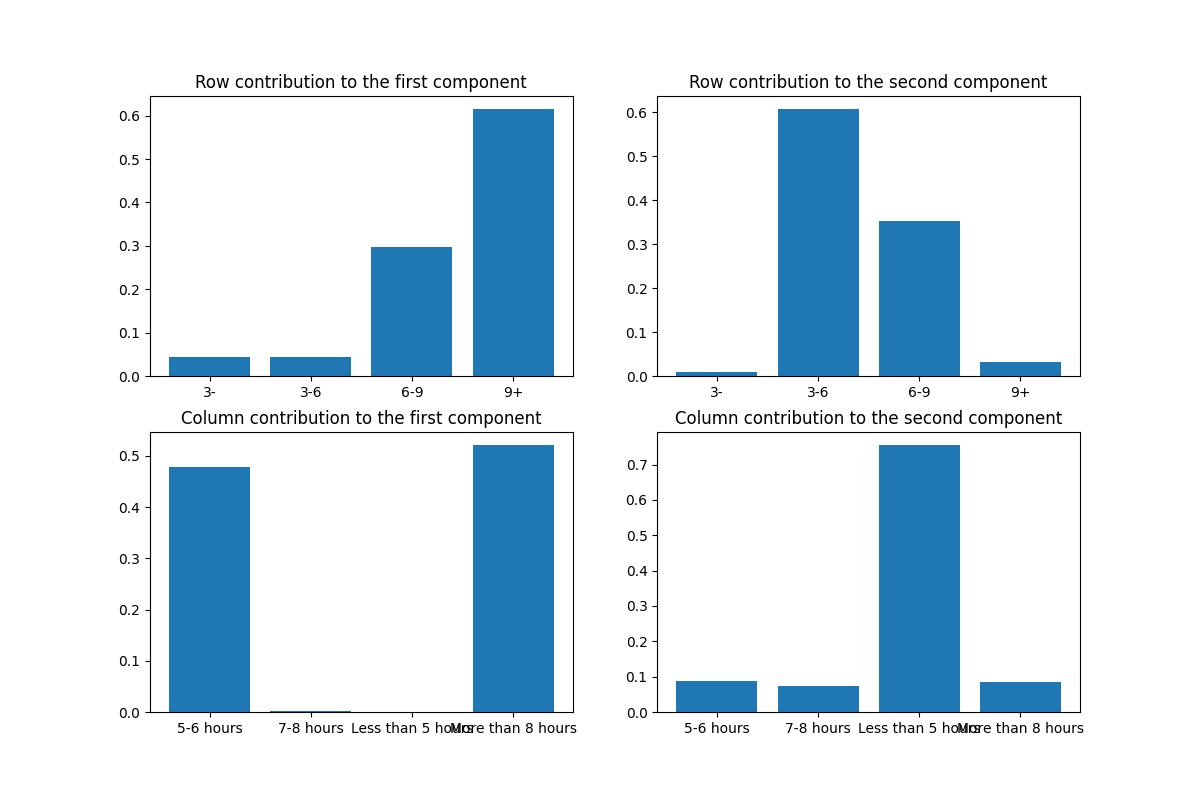
\includegraphics[width=0.65\textwidth]{Images/Study_Sleep_all/RowColumnsContributions.png}
    \end{center}
    \caption{Contribution des catégories de temps d'études et temps de sommeil dans les composantes principales}
    \label{fig:contribStudySleep}
  \end{figure}




